\documentclass[12pt,letterpaper]{article}

%{{{ Package configuration
%%%%%%%%%%%%%%%%%%%%%%%%%%%%%%%%%%%%%%%%%%%%%%%%%%%%%%%%%%%%%%%%%%%%%%%%%%%%%%%%

% Page margin
\usepackage[margin=1in]{geometry}

% Support for bold small cap font
\usepackage[tuenc]{fontspec}
\setmainfont[
    Path=./fonts/,
    Extension=.otf,
    BoldFont=cmu-serif-bold,
    BoldItalicFont=cmu-serif-bold-italic,
    ItalicFont=cmu-serif-italic,
]{cmu-serif}

% Better typesetting quality
\usepackage{microtype}

% Make letter spacing work for both XeLaTeX and LuaLaTeX
\usepackage{ifluatex}
\ifluatex
    \newcommand{\LSSTYLE}{\lsstyle}
\else
    \newcommand{\LSSTYLE}{\addfontfeatures{LetterSpace=12}}
\fi

% Math
\usepackage{amsmath}
\renewcommand{\vec}[1]{\mathbf{#1}}                   % Bold as vector
\newcommand{\spin}[1]{#1}                             % spinor doing nothing
\newcommand{\Lden}[1]{\ensuremath{\mathcal{L}_{#1}}}  % Lagrangian density

% SI units
\usepackage{siunitx}

% Figure
\usepackage{float,graphicx}

% Feynman slash notation
\usepackage{centernot}
\newcommand{\fsl}[1]{\ensuremath{\centernot{#1}}}

% Redefine section, subsection styles
\usepackage[compact,center,explicit]{titlesec}
\usepackage{textcase}
\titleformat{\section}{\LSSTYLE\normalsize\scshape\filcenter}
    {\thesection}{1em}{\MakeTextUppercase{#1}}
\titleformat{\subsection}{\small\bfseries\filcenter}
    {\thesubsection}{1em}{#1}

% PRL-style horizontal rule
\usepackage{amssymb}
\newcommand{\PRLrule}{
    \bigskip
    \noindent\makebox[\linewidth]{
        \resizebox{0.3333\linewidth}{1pt}{$\blacklozenge$}
    }
    \bigskip
}

% Bold math in section title
\makeatletter
\g@addto@macro\bfseries{\boldmath}
\makeatother

% Tabular
\usepackage{booktabs}

% Float barrier
\usepackage{placeins}

% Set up author affiliation
\usepackage[affil-it]{authblk}

% Set up link, with (hopefully) math symbol support
\usepackage[pdfencoding=auto,psdextra]{hyperref}
\hypersetup{colorlinks,breaklinks,citecolor=blue}
\usepackage{cleveref}

% Set up bibliography
\usepackage[
    %style=phys,
    giveninits=true,
    %backref=true,
    natbib=true,
    backend=biber,
    doi=true,
    % Sort by the order of citation
    sorting=none,
    % This options ensures that no automatic et al. is generated
    %maxbibnames=99,
    % This option must be enabled with 'babel' package
    useprefix=false
]{biblatex}
\addbibresource{umd_phd_candidacy_paper.bib}

%}}}

%{{{ User settings
%%%%%%%%%%%%%%%%%%%%%%%%%%%%%%%%%%%%%%%%%%%%%%%%%%%%%%%%%%%%%%%%%%%%%%%%%%%%%%%%

% User-defined variables
\def\BaBar/{\textsc{BaBar}}
\def\Y4S/{\ensuremath{\Upsilon(\text{4S})}}
\def\RD/{\ensuremath{\mathcal{R}(D)}}
\def\RDst/{\ensuremath{\mathcal{R}(D^{*})}}
\def\RDDst/{\ensuremath{\mathcal{R}(D^{(*)})}}
\def\DDst/{\ensuremath{D^{(*)}}}
\def\Dst/{\ensuremath{D^*}}
\def\Dstst/{\ensuremath{D^{**}}}
\def\TauLepMode/{\ensuremath{
    \tau^- \rightarrow \ell^- \nu_\tau \bar{\nu}_\ell
}}
\def\TauHadMode/{\ensuremath{
    \tau^- \rightarrow \pi^- \pi^+ \pi^- \nu_\tau
}}

\newcommand{\BMesonMode}[2]{\ensuremath{
    B \rightarrow #2 #1^- \bar{\nu}_#1
}}

\newcommand{\BDDstMode}[1]{\BMesonMode{#1}{\DDst/}}
\newcommand{\BDstMode}[1]{\BMesonMode{#1}{\Dst/}}
\newcommand{\BDMode}[1]{\BMesonMode{#1}{D}}

% Title info
\title{
    A review of testing lepton flavor universality in semileptonic $B$ decays
}
\author{Yipeng Sun}
\affil{Department of Physics, University of Maryland}
\date{\today}

%}}}

\begin{document}
\maketitle

\begin{abstract}
    The Standard Model expects all leptons couple the same to gauge bosons,
    except the Higgs, a feature called lepton flavor universality.
    However, measurements from the \BaBar/, BELLE, and LHCb experiments show
    tension with this expectation.
    This paper briefly reviews the theoretical foundations of lepton flavor
    universality, the recent results challenging it, and the prospect for a
    resolution.
\end{abstract}

\section{Introduction}
The Standard Model (SM) has been very successful in describing the interactions
between elementary particles such as quarks and leptons.
The theory has been tested experimentally to a very high precision.
However, there are phenomena that cannot be explained by the SM, such as
the observed matter-antimatter asymmetry in the universe and a lack of dark
matter candidate, hinting that there might be New Physics (NP) beyond the SM.
One way to search for NP is to measure the properties of certain processes
very precisely;
properties that differ from the SM predictions may provide evidence for NP.

Through experimental discovery, it has been established that leptons have three
flavors and each flavor has charged and neutral counterparts:
the charged leptons are the electron $e$, muon $\mu$, and tau $\tau$,
with the neutrinos $\nu_e$, $\nu_\mu$ and $\nu_\tau$ being their neutral
partners.
The SM assumes that all three flavors of leptons participate in all
interactions with the same strength, except for the Higgs mechanism through
which they acquire their masses.
This is known as Lepton Flavor Universality (LFU).

LFU has been tested by many precision measurements, such as the decay rate
of $K \rightarrow e^- \bar{\nu}_e$ versus
$K \rightarrow \mu^- \bar{\nu}_\mu$\footnote{
    Unless specified, charge conjugation is assumed throughout the paper.
} \cite{Ciezarek:2017yzh} and the ratio of the leptonic partial widths
$\frac{B(Z \rightarrow \mu^- \mu^+)}{B(Z \rightarrow e^- e^+)}$ versus
$\frac{B(Z \rightarrow \tau^- \tau^+)}{B(Z \rightarrow e^- e^+)}$
\cite{ALEPH:2005ab}, have been performed.
So far, no definite violation of LFU has been detected.

This paper provides a review on recent measurements that challenge LFU
in the semileptonic decays of $B$ mesons, such as
\BDDstMode{\ell} where the \DDst/ denotes a $D$ or \Dst/ meson.
The difference in decay rates in these measurements is typically characterized
by \RDDst/, defined as\footnote{
    $\mathcal{B}$ denotes branching fraction.
    $\ell$ stands for light leptons, namely an $e$ or a $\mu$, but not a $\tau$.
}:
\begin{equation}
    \RDDst/ \equiv \frac{
        \mathcal{B}\left( \BDDstMode{\tau} \right)
    }{
        \mathcal{B}\left( \BDDstMode{\ell} \right)
    }
\end{equation}

Currently, the world average of the combined decay rate ratio \RDDst/
has a $3.08\sigma$ deviation from the SM prediction \cite{HFLAV:2019}, pointing
to a possible lepton flavor universality violation (LFUV);
many collaborations are working on more precise measurements to provide a
definite answer.

In this paper, we begin with a theoretical review on why SM manifests LFU;
Higgs mechanism to show the couplings between different flavors of leptons and
Higgs bosons are different;
extensions to SM such as the 2-Higgs-Doublet Model (2HDM) that may lead to LFUV;
we then review and compare colliders and detectors, such as \BaBar/ at PEP-II
and LHCb at the Large Hadron Collider (LHC), used in testing of LFU.
After that, we will review current experimental results.
Finally, we provide an overview of future measurements for a possible resolution
to current anomalies.

\section{Theory}
\subsection{Lepton flavor universality} \label{sec:lfu}
Leptons participate in electroweak interaction only;
the interaction can be described by a Lagrangian of the following form:
$\Lden{ew} = \Lden{gauge} + \Lden{f} + \Lden{\phi} + \Lden{Yuk}$.
The fermion part of \Lden{ew} reads \cite{Langacker:2010zza}:
\begin{align}
    \Lden{f} = \sum_{l = 1}^F \Big(
        & \bar{\spin{q}}^0_{lL} i \fsl{D} \spin{q}^0_{lL} +
          \bar{\spin{l}}^0_{lL} i \fsl{D} \spin{l}^0_{lL} + \nonumber \\
        & \bar{u}^0_{lR} i \fsl{D} u^0_{lR} +
          \bar{d}^0_{lR} i \fsl{D} d^0_{lR} +
          \bar{e}^0_{lR} i \fsl{D} e^0_{lR} +
          \bar{\nu}^0_{lR} i \fsl{D} \nu^0_{lR}
    \Big)
\end{align}
where the number $F$, empirically 3, of fermion flavors is summed over, and
$L,R$ denote $SU(2)_L$ doublet\footnote{
    The left-handed lepton doublet is defined as:
    $\spin{l}^0_{lL} = \begin{pmatrix} \nu_l \\ l \end{pmatrix}$,
    where $l$ denotes lepton flavor.
}
and singlet in each flavor generation.
From the Lagrangian we see that the interactions between fermions and gauge
bosons (the interactions are embedded in the \fsl{D} operator) is independent
of their flavor.
But this is only an incomplete picture:
Fermions acquire their mass through their interaction with the Higgs bosons,
which is omitted above.

No mass term of the form $m \overline{\Psi} \Psi$ is permitted, since it would
spoil $SU(2)$ symmetry of the Lagrangian\footnote{
    To be precise, \Lden{ew} is locally invariant under the transformations in
    $SU(2)_L \otimes U(1)$ group.
}.
Instead, we add a doublet scalar field $\Phi$ interacting on both gauge bosons
and fermions.
After spontaneous symmetry breaking of the vacuum state, the Lagrangian remains
unbroken, and the new terms in the Lagrangian are interpreted as mass terms.
We inspect the mass terms for the leptons \cite{Langacker:2010zza}\footnote{
    The notation has been simplified.
}:
\begin{equation}
    m_l \equiv \Gamma_l \frac{\nu}{\sqrt{2}}
\end{equation}
with $\nu$ interpreted as vacuum expectation value of $\Phi$.
This shows that leptons coupling stronger to the $\Phi$ (Higgs) field will be
more massive.

This completes the picture.
Now we see that SM demands LFU, except for the Higgs coupling.


\subsection{Higgs mechanism}
However, \autoref{sec:lfu} is only an incomplete picture:
Leptons acquire their mass through their interaction with the Higgs bosons,
but different flavor of leptons have different mass, this implies lepton-Higgs coupling varies with flavor. 

The electroweak Lagrangian is locally invariant under $SU(2)$ transformations;
this symmetry needs to be preserved.
Naive Mass term of the form $m \overline{\Psi} \Psi$
spoils $SU(2)$ symmetry of the Lagrangian, hence it is not permitted.
Instead, we add a doublet scalar field $\Phi$, known as Higgs doublet, interacting on both gauge bosons
and fermions.
After spontaneous symmetry breaking of the vacuum state, the Lagrangian preserves its 
symmetry, and the new terms in the Lagrangian, encapsulated in \Lden{yuk}, are interpreted as mass terms.

We inspect the coupling in the mass terms for the leptons \cite{Langacker:2010zza}\footnote{
    The notation has been simplified.
}:
\begin{equation}
    m_l \equiv \Gamma_l \frac{\nu}{\sqrt{2}}
\end{equation}
with $\nu$ interpreted as vacuum expectation value of $\Phi$, and $\Gamma_l$ the coupling between lepton with flavor $l$ and Higgs.
This shows that leptons coupling stronger to the $\Phi$ (Higgs) field will be
more massive.

The Higgs mechanism completes the picture:
Now we see that SM demands LFU, except for the Higgs coupling.

\subsection{Extensions to SM}
SM assumes that there is only one Higgs-doublet $\Phi$; however, leptons have
three families.
Inspired by the multi-family nature of the leptons, theorists proposed many two
Higgs-doublet models (2HDM) that may violate LFU \cite{Branco:2011iw}.
All 2HDM predict the existence of a charged Higgs $H^{\pm}$, which can have
sizable indirect effects in $B$ physics \cite{Branco:2011iw}.

% type-II model claimed to be excluded; type-III (very similar to type-II) still
% alive.
% Leptoquark is currently the more popular model
The 2013 \BaBar/ paper excluded type-II 2HDM, a minimal extension to the SM, at
95\% confidence level \cite{Lees:2013uzd}.
More complex 2HDM, which induces increasingly deviating predictions from SM, is
still not fully excluded.

Another popular extension to the SM is the leptoquark model, which enables
direct interaction between a quark and a lepton.
This model also permits LFUV \cite{Faber:2018afz}.


\section{Production and detection of $B$ mesons in different experiments}
$B$ mesons have been primarily generated by two types of colliders:
$e^- e^+$ colliders tuned at a center-of-mass energy corresponding to a
$b\bar{b}$ resonance, which are often referred as ``$B$ factories", and hadron
colliders.
We will review $B$ production and detection in detail at \BaBar/ and LHCb,
representing $B$ factory and hadron collider.
BELLE is another $B$ factory that shares most of its features with \BaBar/, so
its details will not be provided.

\subsection{\BaBar/ at PEP-II} \label{sec:babar}
% Talk about PEP-II and its asymmetrical beam energies
PEP-II is an asymmetrical $e^- e^+$ collider at SLAC.
In PEP-II, $B$ mesons are produced primarily in the following process:
$e^- e^+ \rightarrow \Y4S/ \rightarrow B \bar{B}$, with
$e^-$ and $e^+$ beams tuned at different energies,
such that the invariant mass is at the \Y4S/ resonance (\SI{10.58}{GeV}),
and the momentum of the \Y4S/ in the lab frame
non-zero \cite{Harrison:1998yr}.

Producing at \Y4S/ peak eliminates almost all fragmentation products, reducing
combinatorial background.
Also, since the momenta of $e^- e^+$ is known, with the reconstruction of the
momentum of one $B$ meson ($B_{tag}$), the rest frame of the other $B$
($B_{sig}$) can be calculated as
\begin{equation}
    p_{B_{sig}} = p_{e^-e^+} - p_{B_{tag}}.
\end{equation}
Later we will see that this makes identifying events that have more than one
missing particle easier.

% Talk about subdetectors
\BaBar/ is a barrel detector (shown in \autoref{fig:babar_detector_view})
that consists of five subdetectors.
From inside out:
Silicon Vertex Tracker (SVT) and Drift Chamber (DCH), which measure the momenta
and angles of charged particles.
Detector of Internally Reflected Cerenkov radiation (DIRC), together with SVT
and DCH, identifies charged particles of different masses by Cerenkov
ring-imaging and ionization energy loss of these particles.
Caesium Iodide Electromagnetic Calorimeter (EMC), which measures energy and
position of electromagnetic showers generated by electrons and photons.
A superconducting solenoid with a \SI{1.5}{T} magnetic field surrounding the
EMC, together with Instrumented Flux Return (IFR), is used to identify muons and
some neutral hadrons \cite{Lees:2013uzd}.

\begin{figure}[ht]
    \centering
    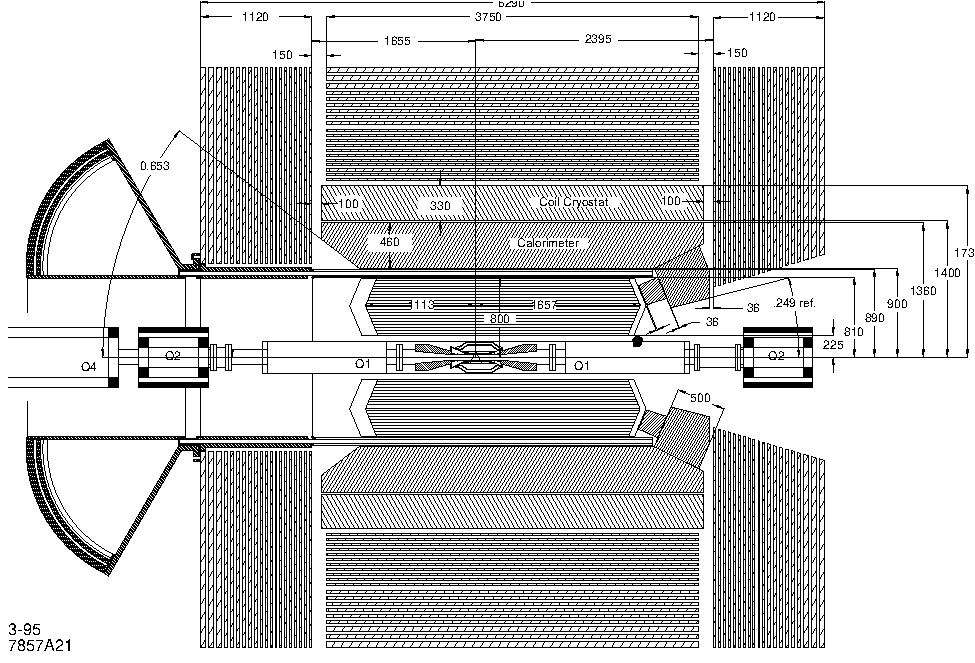
\includegraphics[width=0.7\textwidth]{figs/babar_detector_view.pdf}
    \caption{
        View of the \BaBar/ detector.
        Extracted from \cite{Boutigny:1995ib}.
    }
    \label{fig:babar_detector_view}
\end{figure}

% Talk about BaBar being 4 pi
In $e^- e^+$ detectors, $b \bar{b}$ is produced at all solid angles with
non-negligible probability \cite{Boutigny:1995ib,McGregor:2008ek}, thus the
detector needs to cover almost all solid angles (a $4\pi$ detector).
Indeed, \BaBar/ has tracking coverage of 0.92, namely 92\% of the $4\pi$ solid
angle.

% Talk about tracking and calorimeters
$B$ physics requires excellent vertex resolution and tracking, because the two
$B$ mesons produced by \Y4S/ must be reliably separated.
\BaBar/ has excellent tracking for charged particles, and sufficient spatial
and energy resolution in the electromagnetic calorimeter to reconstruct the
momenta of neutral particles \cite{Bauer:2005} with adequate precision.


\subsection{LHCb at the LHC} \label{sec:lhcb}
The LHC is a $pp$ collider, located at Geneva, Switzerland.
% Talk about the LHC being a hadron collider and the difficulties associated
% with it
Unlike electrons and positrons, the proton is a composite particle made of
$u, u, d$ quarks as well as other virtual partons.
All these particles participate in the $pp$ collision, carrying
varying portion of the total momentum.
The exact fraction of momentum carried by each type of parton is described by
parton distribution function\footnote{
    The parton distribution function is defined as:
    Number density to find fraction of the momentum (denoted as $x$) at certain
    squared energy scale $Q^2$.
} \cite{Ball:2014uwa}.
Since the precise fraction of momentum carried by interacting
partons\footnote{
    Again, these are characterized by parton distribution functions
} is unknown, the $B$ meson rest frame is not readily calculable.

Because many partons, such as quarks and gluons, can interact both
electroweakly and strongly,
the cross section of $b \bar{b}$ is larger than that of the $B$ factories, as a
result, more $b \bar{b}$ events are generated.
The measured $b \bar{b}$ cross section at LHCb in \SI{13}{TeV} $pp$
collisions\footnote{
    For $2 < \eta < 5$ only, since this is the LHCb acceptance range.
} is $144 \pm 1 \pm 21$~\si{\mu b} \cite{Aaij:2016avz}, whereas at the $B$
factories it is only about $1.05$~\si{nb} \cite{Harrison:1998yr}.
At the same time, unwanted particles will be generated frequently at hadron
colliders, leading to higher background.


% Talk about subdetectors
LHCb, a single-arm spectrometer, is one of the four large experiments at the
LHC.
Its constituent subdetectors, from closest to farthest from the collision point,
are shown in \autoref{fig:lhcb_detector_view}:
The Vertex Locator (VELO) provides precise measurements of track coordinates
close to the collision point.
Two Ring Imaging Cerencov counters (RICH1, RICH2) provide particle
identification for charged particles over a wide range of momentum.
The Tracker Turicensis (TT), Inner Tracker (IT), and Outer Tracker (OT) provide
additional tracking for charged particles and measure their momenta.
The calorimeters (ECAL and HCAL) have a first-level (L0) trigger to select
hadron, electron, and photon candidates based on their transverse momentum
$p_T$;
they also provide identification for the particles listed above;
finally, they provide energy and position measurements for these particles.
The Muon system (M1-5) is farthest from the collision point;
it provides L0 high $p_T$ muon trigger, and a high-level trigger (HLT) for muon
identification. Compared to the $B$ factories, LHCb has a much lower trigger
efficiency, which means many interesting events are filtered
out \cite{LHCb:2008}.

\begin{figure}[ht]
    \centering
    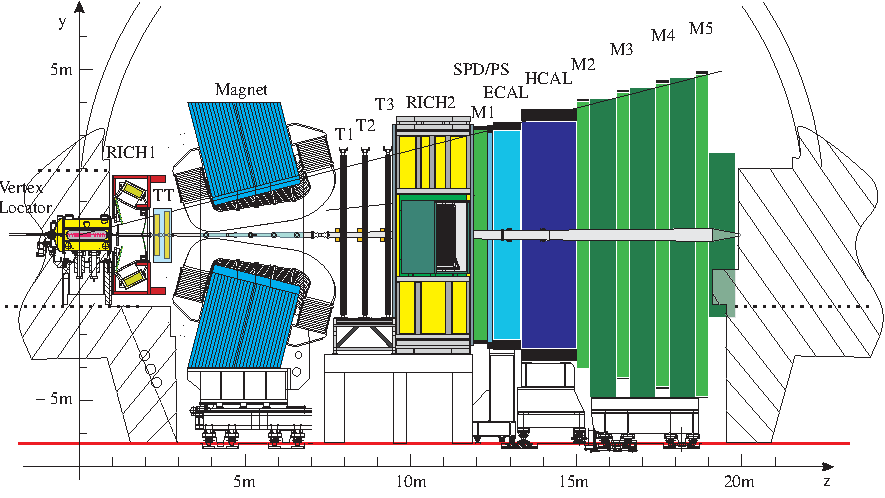
\includegraphics[width=0.7\textwidth]{figs/lhcb_detector_view.pdf}
    \caption{
        View of the LHCb detector and its subsystems.
        Extracted from \cite{LHCb:2003ab}.
    }
    \label{fig:lhcb_detector_view}
\end{figure}

% Talk about LHCb being forward-only
An interesting design choice is the geometry of the LHCb detector:
Instead of being a barrel $4\pi$ detector, it is forward-only.
This is because at high energies, $b\bar{b}$ is mostly produced in the forward
and backward direction.
The LHCb design is a very cost-effective way to construct a detector at the LHC
dedicated for $B$ physics.

% Talk about tracking
LHCb has a very good vertexing and tracking system, achieving vertex resolutions
down to 20~$\mu$m in a challenging environment.
However, due to the amount of material before the calorimeters and their poor
granularity,
reconstruction of neutral particles, such as $\pi_0$, is less
precise \cite{LHCb:2008,Guz:2017}.
This is why LHCb analyses typically focus on final states with charged particles
only, whereas $B$ factories can afford to use final states with neutral
particles.

% Talk about run 1 and run 2 luminosity
LHCb collected data from 2010 to 2012 with a center of mass energy of
\SI{8}{TeV}, and from 2015 to 2018 at \SI{13}{TeV}.
The total integrated luminosity during these two periods is about
\SI{9.2}{fb^{-1}} \cite{LHCb-Lumi:2019}.
% Talk about LS2 upgrade and LHCb's future
Currently, LHCb is shut down for an upgrade which will greatly increase the
readout rate of the detector starting in 2021.


\section{Current measurements of \RDDst/}
In 2013, \BaBar/ reported a $3.4\sigma$ discrepancy in \RDDst/ from the
theoretical predictions \cite{Lees:2013rw}.
Since then, follow up measurements on the same semileptonic channel have been
performed by \BaBar/, BELLE, and LHCb, reporting various degrees of
discrepancies \cite{Hirose:2017185, LHCb:PhysRevLett.115.111803, Aaij:2017deq}.
The measured results are shown in \autoref{tab:results}.
Currently, the world average of the measured \RDDst/ has a deviation of
$3.08\sigma$ with respect to SM prediction \cite{HFLAV:2019}, as shown
in \autoref{fig:rdrds_spring2019}.

\begin{figure}[ht]
    \centering
    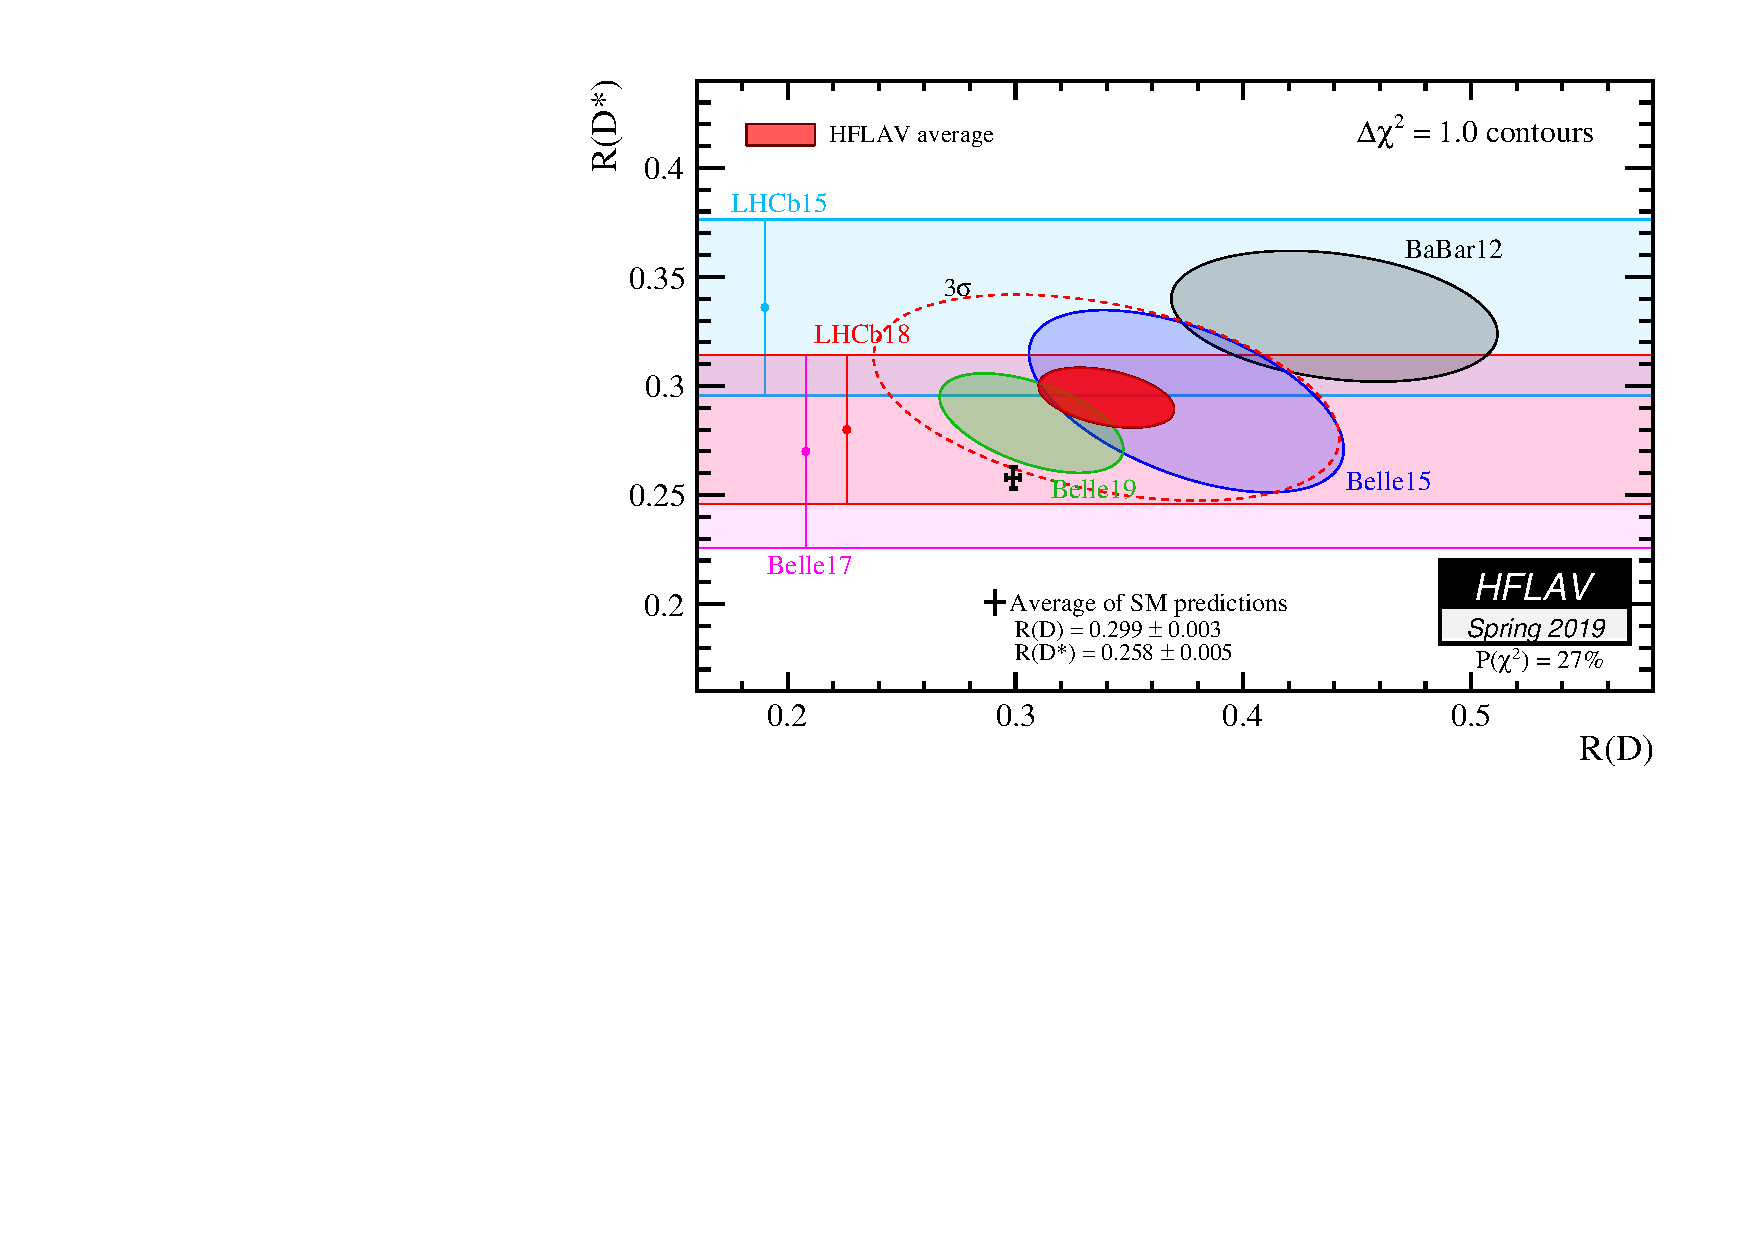
\includegraphics[width=0.6\textwidth]{figs/rdrds_spring2019.pdf}
    \caption{
        World average of measured \RD/ and \RDst/, and SM predictions, as of
        spring 2019 \cite{HFLAV:2019}.
    }
    \label{fig:rdrds_spring2019}
\end{figure}

\begin{table}[ht]
    \centering
    \caption{
        \RDDst/ measurements from $B$ factories and LHCb \cite{HFLAV:2019}.
    }
    \label{tab:results}
    \vspace{1em}
    \begin{tabular}{lll}
        \toprule
        Experiment  &  \RDst/                               &  \RD/                         \\
        \midrule
        \BaBar/     &  $0.332 \pm 0.024 \pm 0.018$          &  $0.440 \pm 0.058 \pm 0.042$  \\
        BELLE       &  $0.293 \pm 0.038 \pm 0.015$          &  $0.375 \pm 0.064 \pm 0.026$  \\
        LHCb        &  $0.336 \pm 0.027 \pm 0.030$          &  -                            \\
        BELLE       &  $0.270 \pm 0.035^{+0.028}_{-0.025}$  &  -                            \\
        LHCb        &  $0.280 \pm 0.018 \pm 0.029$          &  -                            \\
        BELLE       &  $0.283 \pm 0.018 \pm 0.014$          &  $0.307 \pm 0.037 \pm 0.016$  \\
        \bottomrule
    \end{tabular}
\end{table}

\subsection{Measurements at the $B$ factories} \label{sec:meas_bfactories}
The $B$ factories reconstruct \BDDstMode{\tau} (signal) and \BDDstMode{\ell}
(normalization) decays by selecting events with a tagged $B$ meson ($B_{tag}$),
a \DDst/ meson, and an $e$ or $\mu$.
As described in \autoref{sec:babar}, the $B$ factories can estimate the momenta
of the $B \overline{B}$ system precisely by tagging and reconstructing the other
$B$, known as $B_{tag}$.
By subtracting the momentum of $B_{tag}$ to that of initial $e^-e^+$ system, the
momentum of the signal $B_{sig}$, which decays semileptonically and thus
contains unreconstructed neutrinos in the final state, can be inferred.

\BaBar/ and BELLE independently developed two types of tagging algorithms:
semileptonic tagging and hadronic tagging.
Semileptonic tagging finds $B_{tag}$ with the following decay: \BDDstMode{\ell}.
This has the advantage of a larger branching ratio, thus more ($\approx 1\%$)
\Y4S/ events are tagged.
However, in this type of events, the $B_{tag}$ side has at least one missing
neutrino, which makes the reconstruction of $p_{B_{sig}}$ less
precise \cite{Ciezarek:2017yzh}.

On the other hand, hadronic tagging searches over a very large number of
hadronic decay chains of $B$ for each \Y4S/ event, tagging the ones that match
one of the known modes.
This has a smaller tagging rate ($\approx 0.3\%$), but because $B_{tag}$ decays
hadronically, no missing neutrino is present in the tagged final product.
This makes the reconstructed momentum of $B_{sig}$ very
precise \cite{Lees:2013uzd,Ciezarek:2017yzh}.

$D^{0}$ and $D^{+}$ mesons are reconstructed in numerous final states, including
final states with neutral particles.
$D^{*0}$ and $D^{*+}$ mesons are reconstructed by associating soft pions or
photons with previously reconstructed $D$ mesons.

All $B$ factory measurements choose a particular decay mode of the $\tau$:
\TauLepMode/.
In this way, the signal and the normalization \BDDstMode{\ell} decays are
reconstructed in the same final state, leading to the cancellation of several
sources of experimental uncertainty in the \RDDst/ ratios.
While both signal and normalization events have the same visible particles in
the final state, the signal mode has three neutrinos in the final product,
whereas the normalization mode has only one.
By looking at the missing mass of the $B_{sig}$, defined as
\begin{equation}
    m^2_{miss} \equiv \left(p_{B_{sig}} - p_{visible}\right)^2,
\end{equation}
the signal, which has a non-zero $m^2_{miss}$, can be readily differentiated
from the normalization, which does have a $m^2_{miss} \approx 0$.

Non-$B \overline{B}$ background and misreconstructed events are suppressed by
rejecting events with tracks that are not used in the reconstruction of the
$B_{tag}$, \DDst/, or lepton.

The main background remaining is due to semileptonic
\BMesonMode{\ell}{\Dstst/} decays.
\Dstst/ decays into a \Dst/ and a number of soft pions, which are often not
reconstructed.
As a result, the $m^2_{miss}$ distribution is similar to that of the signal.
This background is constrained by constructing $\DDst/ \pi^0 \ell$ control
samples with the same selection as the signal samples plus an additional
$\pi^0$.
In these control samples, \Dstst/ mesons that decay to $\DDst/ \pi^0$ are
fully reconstructed, leading to an easily distinguishable peak in the
$m^2_{miss}$ distribution.

The signal and normalization yields are extracted from maximum-likelihood fits,
which rely primarily on the $m^2_{miss}$ and $|\vec{p}^*_\ell|$ distributions.
The fit result is shown in \autoref{fig:babar_lhcb_fit_comparison}.
The probability distribution functions for all contributions are taken from
Monte-Carlo simulated samples, with corrections coming from data control
samples.

As can be seen in \autoref{tab:results}, all four $B$ factory results are
limited by the size of their data samples.


\subsection{Measurements at LHCb} \label{sec:meas_lhcb}
% 2015 LHCb leptonic tau decay
LHCb has published two measurements of \RDst/; one measurement from 2015 where
the $\tau$ is reconstructed leptonically in the
$\tau^- \rightarrow \mu^- \bar{\nu}_\mu \nu_\tau$ decay mode,
and another from 2018 where the $\tau$ is reconstructed in the
$\tau^- \rightarrow \pi^- \pi^+ \pi^- \nu_\tau$ decay.

The 2015 result constituted the first \RDst/ measurement in the very challenging
environment of a hadron collider.
This analysis is heavily inspired by the previous $B$ factory measurements, with
a few key differences:

\begin{itemize}
    \item The $B \overline{B}$ rest frame is unknown.
    \item Larger backgrounds, especially a significant contribution due to the
        following decay mode: $B \rightarrow D^* H_c X$, where $H_c$ is any
        charm meson, and $X$ is any hadronic particle.
        These decay modes have similar $m^2_{miss}$ and $E^{*}_l$ distributions
        very similar to the signal.
    \item A particular decay mode of the $B$ and $D^{*}$ are chosen so that all
        visible final state particles are charged due to the fact that the
        neutral particle resolution is not very good.
\end{itemize}

Without the $B \overline{B}$ rest frame, the tagging algorithms used in the $B$
factory measurements cannot be applied.
This problem is solved by the so-called \emph{rest frame approximation}, a
technique developed specifically for this analysis.
This approximation assumes the momentum of the $B$ that is orthogonal to the
beam axis, transverse momentum, is unchanged.
The component of the $B$ momentum parallel to the beam axis, $(p_{B})_z$, is
approximated as
\begin{equation}
    (p_{B})_z = \frac{m_B}{m_{reco}} (p_{reco})_z,
\end{equation}
with $m_B$ being the known $B$ mass, and $reco$ referring to the $D^{*+} \mu^-$
system.
The resulting $m^2_{miss}$ resolution is worse than that of the $B$ factories,
but is sufficient to preserve the discriminating power between the signal and
normalization, as shown in \autoref{fig:babar_lhcb_fit_comparison}.

A multivariate method is employed to determine which tracks are likely to have
originated from the $B_{sig}$ decay.
Events that contain tracks that are unassociated with the $D^{*+}$ or the
$\mu^-$ are rejected, reducing the $B \rightarrow D^* H_c X$ and other
backgrounds.
By inverting the isolation selecting criteria, control samples are obtained to
correct for the shape of these background distributions.

An extended, binned, maximum likelihood method is used in the fit, with three
dimensional templates in the $m^2_{miss}$, $E^*_\mu$, and $q^2$ variables
describing the contributions from signal, normalization, and background events.
\autoref{fig:babar_lhcb_fit_comparison} (g, h, i) show the fit results.
We see that this LHCb result has a lower signal-to-background ratio, but
significantly higher number of signal events.

\begin{figure}[ht]
    \centering
    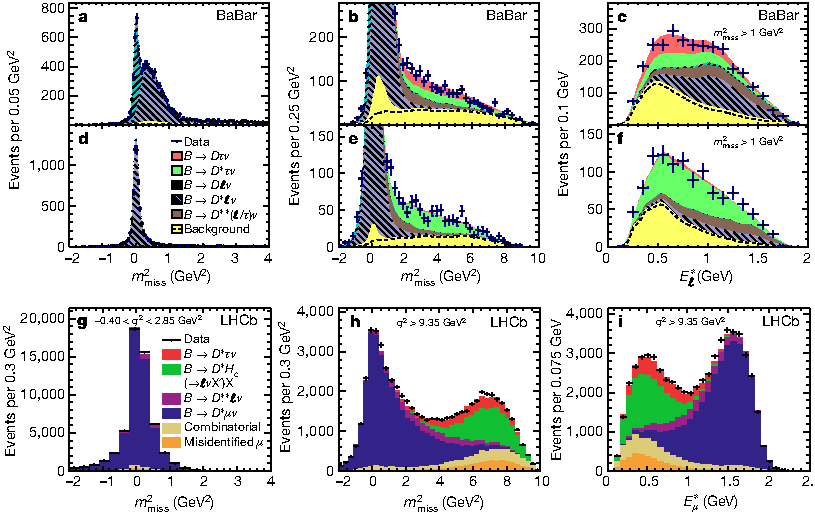
\includegraphics[width=0.85\textwidth]{figs/babar_lhcb_fit_comparison.pdf}
    \caption{
        Comparison between fitted data from \BaBar/ and 2015
        LHCb \cite{Ciezarek:2017yzh}.
    }
    \label{fig:babar_lhcb_fit_comparison}
\end{figure}

% 2018 LHCb hadronic tau decay: tau -> pi pi pi
The 2018 LHCb \RDst/ measurement pioneered the usage of
$\tau^- \rightarrow \pi^- \pi^+ \pi^- \nu_\tau$
decay modes in $B \rightarrow D^{*} \tau \nu_\tau$.

Since the $tau$ lepton is reconstructed with the
$\tau^- \rightarrow \pi^- \pi^+ \pi^- \nu_\tau$ modes, the final state particles
of signal events are different from those of normalization events.
Instead, to cancel experimental systematic uncertainties, this analysis employs
the $B^0 \rightarrow D^{*-} 3\pi$ as the normalization, which has the same final
state particles as that of the signal.
This analysis measures the ratio, defined as $\mathcal{K}(D^{*-}))$
\begin{equation}
    \mathcal{K}(D^{*-}) \equiv \frac{
        \mathcal{B}(B^0 \rightarrow D^{*-} \tau^+ \nu_\tau)
    }{
        \mathcal{B}(B^0 \rightarrow D^{*-} 3 \pi)
    },
\end{equation}
which can be converted back to \RDst/ with the appropriate branching fractions.

This analysis took a different approach to separate signal from normalization
events:
With the decay mode $\tau^- \rightarrow \pi^+ \pi^- \pi^+ \nu_\tau$,
the $\tau$ decay vertex can be reconstructed from the intersection of the three
charged pion tracks.
Due to the non-zero lifetime of the $\tau$, its decay vertex is separated from
the $B$ meson decay vertex.
In contrast, the three pions from the $B \rightarrow D^* \pi \pi \pi X$
normalization (prompt) mode come directly from the $B$ decay vertex.
By requiring a clear separation between the two vertices, the normalization mode
can be effectively separated from signal events, as \autoref{fig:lhcb_3pi_topo}
shows.
The main background is composed of $B \rightarrow D^* D X$ double-charm events,
which is suppressed by a specifically-designed multivariate method.

\begin{figure}[ht]
    \centering
    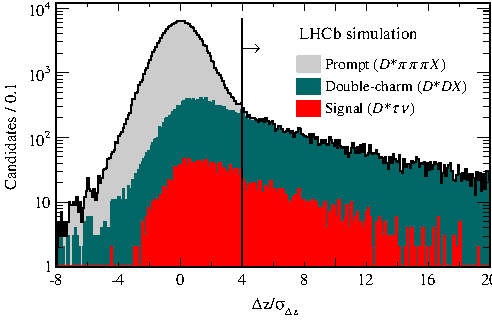
\includegraphics[width=0.65\textwidth]{figs/lhcb_3pi_topo.pdf}
    \caption{
        Separations between the $B$ decay vertex and a secondary vertex, possibly
        $\tau$ decay vertex, in the signal, the normalization, and the
        background decay mode, indicating different topologies between these
        modes \cite{Aaij:2017deq}.
    }
    \label{fig:lhcb_3pi_topo}
\end{figure}

This measurement, which uses the hadronic $\tau$ decays, results in a
significantly reduced statistical uncertainty compared to the 2015 LHCb result.
However the total uncertainty is dominated by systematic effects.


\section{Outlook}
The testing of LFU remains an outstanding problem in precision
physics.
More measurements are needed before any final conclusion can be drawn.
As seen in \autoref{tab:results}, the total uncertainties of $B$ factory
measurements are dominated by their statistical uncertainties.
In the hope to mitigate this problem, BELLE has recently upgraded their
facilities and aim to take a data sample with an integrated luminosity 50 times
larger than that of the previous $B$ factories \cite{Abe:2010gxa}.

In addition to the measurements from $B$ factories, it is crucial to have
independent validations from LHCb, an experiment that has very different sources
of systematic uncertainties.
It is expected that LHCb will publish their first combined \RD/ and \RDst/
measurements in the near future based on the \SI{8}{TeV} dataset
(\SI{3.2}{fb^{-1}}).
Additionally, an update of this measurement based on the \SI{13}{TeV} dataset
(\SI{6.0}{fb^{-1}}) has begun.
% Expected improvements
% Remember: Run 2 supposedly has better pile-ups.
% Current progress
The number of signal events is expected to increase significantly, thanks to
higher integrated luminosity, a larger $b \bar{b}$ production cross section, and
a new dedicated trigger.
An preliminary study shows that the gain might be as high as a factor of 5 per
fb$^{-1}$, as shown in \autoref{fig:lhcb_run2}.
%This is deemed optimistic, and more work is needed to validate the claim.

\begin{figure}[ht]
    \centering
    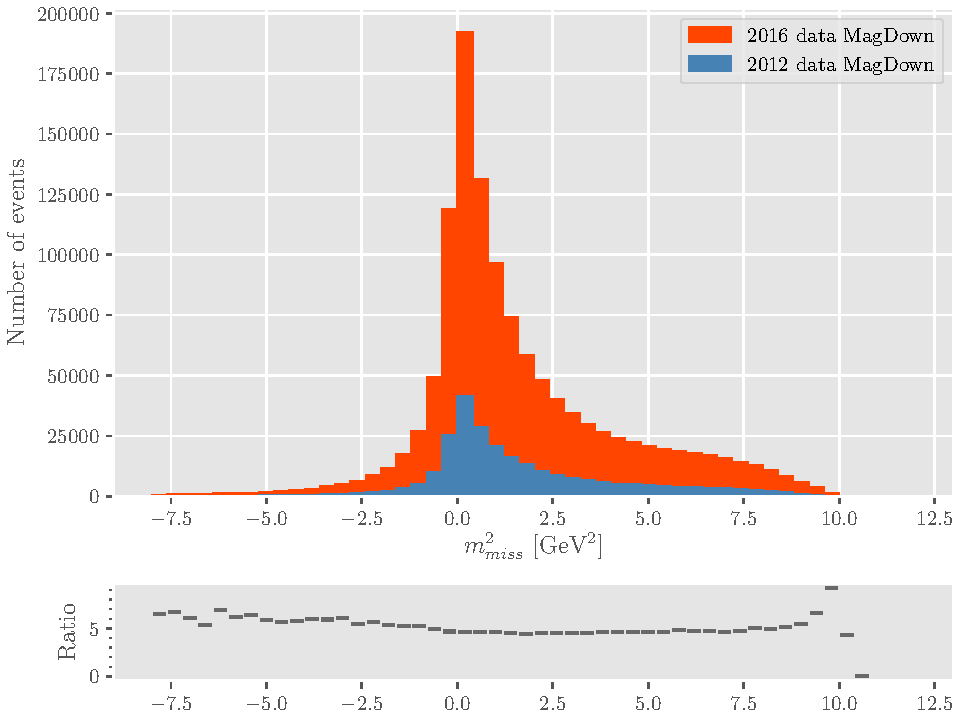
\includegraphics[width=0.6\textwidth]{figs/lhcb_run2.pdf}
    \caption{
        Preliminary study of the comparison between \SI{8}{TeV} and \SI{13}{TeV}
        LHCb data;
        the blue component corresponds to a subset of \SI{8}{TeV} data from 2012
        (\SI{0.99}{fb^{-1}});
        the red to a subset of \SI{13}{TeV} data from 2016 (\SI{0.84}{fb^{-1}}).
        Unpublished result.
    }
    \label{fig:lhcb_run2}
\end{figure}

If NP exists and were to affect the \BDDstMode{\tau} decays, other $B$ decays
with the same $b \rightarrow c \tau^- \bar{\nu}_\tau$ transition should also be
impacted.
Examples include $B_c \rightarrow J/\Psi \ell^- \bar{\nu}_\ell$ and
$\Lambda_b \rightarrow \Lambda_c \ell^- \bar{\nu}_\ell$.
Recent result \cite{Aaij:2017tyk} found tension in the former, and measurements
are in preparation for the latter.
Given all the upcoming measurements from the upgraded BELLE and LHCb, a
resolution to of present anomalies should be achievable in the next few years.

\FloatBarrier
\PRLrule
\printbibliography
\end{document}
